\documentclass[runningheads]{llncs}
\usepackage{graphicx}
\usepackage{booktabs}
\usepackage{amsmath}

\begin{document}

\title{Explainability Fidelity and Deployment Cost in a Trustworthy Cervical Cytology Screening Pipeline}
\titlerunning{Explainability Fidelity and Deployment Cost in Cytology Screening}

\author{Anonymous Author(s)}
\authorrunning{Anonymous Author(s)}
\institute{Submitted for double-blind review}

\maketitle

\begin{abstract}
``Trustworthy AI'' is usually evaluated as if it were one property a
pipeline either has or lacks. We show instead that it decomposes into at
least three independently-varying claims -- which explainability method
is most faithful, whether combining two uncertainty signals improves
selective prediction, and whether an efficient architecture's efficiency
claim holds under real measurement -- and that each one resolves
differently: cleanly, conditionally, or only under direct measurement.
Testing all three side by side on one cervical cytology screening
pipeline, rather than picking one and assuming the others follow the same
pattern, is itself the point. First, we compare three explainability
methods (relevancy propagation, attention rollout, and Grad-CAM adapted
for vision transformers) against both behavioral faithfulness
(deletion/insertion) and a real, expert-annotated localization ground
truth (nucleus boundaries from the SIPaKMeD dataset); relevancy
propagation wins cleanly on all three metrics, with no method-ranking
flip across conditions. Second, we test whether composing two
independently-useful uncertainty signals -- temperature-scaled confidence
and conformal prediction-set size -- into one abstention rule helps: the
answer is conditional, helping exactly where the better individual signal
was already struggling (under severe distribution shift) and hurting
where it was already excellent (in-distribution and under mild shift).
Third, we measure what trustworthiness costs in practice: resource-
efficiency claims for lightweight vision transformers, evaluated by
parameter count and FLOPs alone, do not reliably predict real CPU
inference latency, and returning an explanation alongside a prediction
costs roughly 3.3$\times$ a bare forward pass on CPU. The pattern across
all three -- a clean answer, a conditional answer, and an answer that
only exists once measured -- is the paper's central argument: a single
verification strategy (pick the best method once, assume composition
helps, trust an architectural efficiency claim) does not work uniformly
across a trustworthy-AI pipeline, and each property needs its own,
independent test.

\keywords{Explainable AI \and Vision transformers \and Selective prediction \and Conformal prediction \and Cervical cytology \and Resource efficiency}
\end{abstract}

\section{Introduction}

Cervical cancer screening in specialist-scarce settings is a plausible
target for lightweight, on-device AI assistance, but a screening tool that
fails silently -- misclassifying confidently under conditions its
training data didn't cover -- is more dangerous than one that fails and
says so. Prior work established that a lightweight hybrid vision
transformer (EfficientViT-M0) matches or exceeds much larger CNN and
full-size ViT baselines on in-distribution cervical cytology accuracy, and
that this same backbone can collapse to near-chance accuracy under
cross-dataset distribution shift with no static architectural property
predicting which models fail safely. A companion study asked whether any
of four uncertainty-quantification methods' native confidence signals
correctly flag that collapse, and found a genuinely mixed answer: MC
Dropout's entropy signal is the only one that substantially improves
shift-failure detection on the severe shift condition, while a deep
ensemble -- the best method in-distribution and under mild shift -- does
not transfer that advantage to the severe case.

These two prior findings already show that no single fixed choice
(backbone, uncertainty method) is safe across all conditions -- but each
paper tested only one property of the pipeline. The question this paper
asks is broader: if trustworthiness is not one property but several, do
they all fail to compose the same way, or does each one behave
differently under scrutiny? We answer this by testing three additional
properties of the same pipeline side by side, deliberately choosing
properties that a reader might otherwise assume behave alike:
\textbf{explainability method choice} (does picking the best
explainability method matter as much, and in the same
condition-dependent way, as picking the best uncertainty method?),
\textbf{uncertainty-signal composition} (given that no single uncertainty
method is reliably best, does \emph{combining} two different native
signals into one system help, or does composition just average away
whichever signal was better?), and \textbf{measured deployment cost} (does
a lightweight-architecture claim, evaluated only by parameter count and
FLOPs, actually hold once CPU latency and the cost of an explanation are
measured directly?). The answers turn out to differ in kind, not just in
degree: explainability method choice resolves cleanly to one winner
across all metrics tested; signal composition resolves conditionally,
flipping between helpful and harmful depending on shift severity; and the
deployment-cost claim resolves only once measured, contradicting what
parameter count and FLOPs alone would predict. This three-way divergence
-- not any single result -- is this paper's contribution: it demonstrates
that a trustworthy-AI pipeline cannot be verified with one strategy
applied uniformly to every component.

Our contributions are threefold, one per property tested. First, a
three-way explainability comparison (relevancy propagation vs.\ attention
rollout vs.\ Grad-CAM) on deletion/insertion faithfulness \emph{and} real
expert-annotated nucleus-localization ground truth, where relevancy
propagation wins unambiguously on all three metrics -- a cleaner result
than either companion study's uncertainty-method comparisons produced,
and evidence that this property, at least, does not need the
condition-by-condition re-testing the other two do. Second, the first
system-level test of whether combining two uncertainty signals for
selective prediction helps: a conditional answer (helps under severe
shift, hurts in-distribution and under mild shift) that extends the ``no
single best method'' finding from individual methods to method
combinations, and shows that composition is not a safe default even when
each signal alone is well understood. Third, a measured, not estimated,
resource-efficiency and deployment-cost analysis: parameter count and
FLOPs do not reliably predict CPU latency across a 12-model registry, and
an explanation costs $\sim$3.3$\times$ a bare forward pass -- a reminder
that even the most ``static'' of the three properties tested here still
required direct measurement, not architectural reasoning, to characterize
correctly.

\section{Related Work}

\subsection{Transformer explainability methods}

Attention rollout \cite{abnar2020quantifying} treats a transformer's own
attention weights, chained across layers via a fixed recurrence, as a
relevance signal, on the premise that attention indicates where a model
``looks.'' This premise has itself been contested in the broader
literature examining whether attention weights are faithful explanations
of a model's actual decision process rather than merely correlated with
it -- a concern this paper's own faithfulness metrics (Section~3.3) are
designed to test empirically rather than assume either way. Relevancy
propagation \cite{chefer2021transformer} extends attention rollout by
weighting each transformer block's attention matrix with its gradient
with respect to the target class before the same rollout aggregation,
making the resulting relevance map class-discriminative rather than a
fixed structural property of attention, and is the primary method
evaluated here specifically because it addresses the class-agnosticity
critique of raw attention directly. Grad-CAM \cite{selvaraju2017gradcam}
was originally designed for CNN feature maps, where a single late
convolutional layer naturally encodes class-relevant spatial structure;
its adaptation to transformers by targeting a block's token-wise
activations instead of a convolutional feature map is common practice in
the literature, but the specific failure mode we identify and document
(Section~3.2) for CLS-token-pooled ViTs -- an all-zero heatmap if the
wrong block is targeted -- does not appear to be widely flagged in prior
adaptations, despite being silent rather than an error.

\subsection{Selective prediction and conformal calibration}

Split conformal prediction provides a distribution-free, finite-sample
coverage guarantee from a single calibration split, at the cost of
producing a set of plausible labels rather than one score; its prediction
set size is a natural, model-agnostic uncertainty proxy, but one that is
coarse (a small integer count) compared to a continuous confidence score.
MC Dropout \cite{gal2016dropout}, deep ensembles
\cite{lakshminarayanan2017ensembles}, and evidential deep learning
\cite{sensoy2018evidential} are the three uncertainty-quantification
methods our companion study compares against temperature-scaled softmax;
this paper's system-integration question -- whether combining
temperature-scaled confidence with conformal set size outperforms either
alone -- is, to our knowledge, not directly addressed by prior work
proposing either signal independently, since each is typically evaluated
as a self-contained method rather than as one input to a combined
abstention rule.

\subsection{Faithfulness evaluation}

Deletion/insertion faithfulness \cite{petsiuk2018rise} evaluates an
explanation by its behavioral effect on the model itself (does removing
or revealing the patches an explanation calls important actually change
the model's prediction), rather than by agreement with a human-annotated
region, and is the behavioral-faithfulness metric used throughout this
paper. Evaluating localization against SIPaKMeD's own expert-marked
nucleus polygons, rather than a segmentation model's derived output,
avoids compounding this paper's explainability evaluation with a second
model's own errors.

\subsection{Closely related prior work}

Directly adjacent to this paper's own scope: a stacking-ensemble approach
combined with explainable AI for cervical cancer diagnosis
\cite{mohiuddin2025}, which this paper differs from by evaluating
explainability methods against a real expert-annotated localization
ground truth and behavioral faithfulness metrics rather than an
ensemble-accuracy framing; and a lightweight-ViT-plus-explainability
design for plant disease diagnosis, ``MaizeFormerX''
\cite{rahman2026maizeformerx}, which motivates this paper's own choice to
hold efficiency and explainability as joint, not competing, design goals.
Two further papers sit in adjacent clinical-AI territory: a
semi-supervised retinal disease recognition system
\cite{gony2026retinal} and an explainable multimodal AI framework with
reinforcement learning for post-surgical clinical decision support
\cite{ahmed2026postsurgical}, both part of a broader body of work in
trustworthy, explainable clinical AI of which this paper's cervical
cytology system is one instance.

\section{Methods}

\subsection{Backbone}

The winning in-distribution backbone from our prior efficiency benchmark,
EfficientViT-M0, uses a hybrid convolutional + cascaded-group-attention
design. Relevancy propagation and attention rollout are both defined for
standard multi-head self-attention transformer blocks; EfficientViT-M0 has
no established propagation rule for either method. Rather than force an ad
hoc extension onto an architecture these methods were not designed for,
this paper uses \textbf{DeiT-Tiny} \cite{touvron2021deit} -- a standard
\texttt{timm} \texttt{VisionTransformer} achieving 0.9606 balanced
accuracy on the same SIPaKMeD in-distribution task in our prior benchmark
(vs.\ EfficientViT-M0's 0.9654) -- retrained fresh for this paper.

\subsection{Explainability methods}

All three methods produce a relevance map over the model's 14$\times$14
patch grid (DeiT-Tiny, 224px input, 16px patches), upsampled to image
resolution. \textbf{Attention rollout}: raw softmax attention, averaged
over heads, chained across all 12 blocks via the standard rollout
recurrence. Class-agnostic. \textbf{Relevancy propagation}: identical
rollout recurrence, but each block's contribution is
$\mathrm{ReLU}(\nabla_{\text{attn}} \odot \text{attn})$, averaged over
heads, where the gradient is with respect to the model's own predicted
class's logit. Class-discriminative. \textbf{Grad-CAM (ViT-adapted)}:
gradient-weighted channel importance applied to a transformer block's
token activations rather than a CNN's convolutional feature map.
\emph{Implementation note}: the target layer must be the
\emph{second-to-last} transformer block, not the last. DeiT-Tiny pools
only the CLS token for classification, so no layer downstream of the
final block mixes information back into patch-token positions --
verified directly by inspecting gradients: every patch token's gradient
at the last block's output was exactly zero, while the second-to-last
block's patch-token gradients vary normally.

\subsection{Faithfulness and localization metrics}

\textbf{Deletion/insertion AUC} \cite{petsiuk2018rise}: patches are ranked
by a method's own relevance score and progressively replaced with
(deletion) or revealed from (insertion) a heavily Gaussian-blurred version
of the image, tracking the model's predicted-class probability at each
step; the area under the resulting probability-vs-fraction curve is
reported (lower is better for deletion, higher is better for insertion).
\textbf{Nucleus concentration ratio}: SIPaKMeD ships real, expert-marked
nucleus boundary polygons per cell; we persist these in crop-local pixel
coordinates and compute the fraction of a heatmap's total relevance mass
falling inside the nucleus region, divided by the nucleus's share of
image area. A ratio of 1.0 is exactly chance level; higher values mean a
heatmap concentrates relevance in the nucleus more than chance would
predict -- clinically the correct place to concentrate.

\subsection{Calibration, conformal prediction, and the combined selective-prediction signal}

Temperature scaling \cite{guo2017calibration} is fit on a held-out
calibration split disjoint from both training and test data. Conformal
prediction sets are built via a resampling-averaged split-conformal
threshold. The combined selective-prediction signal rank-normalizes
temperature-scaled max-softmax confidence and (inverted) conformal
prediction-set size independently, then averages their ranks.

\subsection{Efficiency and latency measurement}

Parameters and FLOPs (via \texttt{torch.utils.flop\_counter.FlopCounterMode})
are architecture properties independent of trained weight values, so
measured without any training. CPU latency and memory (isolated per model
in its own subprocess) are measured with untrained weights for the same
reason. The ``cost of an explanation'' is measured as a full
forward+backward+rollout pass for relevancy propagation's own
predicted-class explanation, against a bare forward pass, both on CPU.

\section{Experiments}

\subsection{Explainability results}

\begin{table}[htbp]
\centering
\caption{Explainability method comparison, 50 SIPaKMeD test images, all matched to a real nucleus polygon.}
\label{tab:rq3}
\begin{tabular}{lrrr}
\toprule
Method & Deletion AUC$\downarrow$ & Insertion AUC$\uparrow$ & Nucleus conc.$\uparrow$ (1.0 = chance) \\
\midrule
\textbf{Relevancy propagation} & \textbf{0.734} & \textbf{0.970} & \textbf{2.714} \\
Grad-CAM (ViT-adapted) & 0.818 & 0.877 & 1.472 \\
Attention rollout & 0.825 & 0.936 & 1.177 \\
\bottomrule
\end{tabular}
\end{table}

\begin{figure}[htbp]
\centering
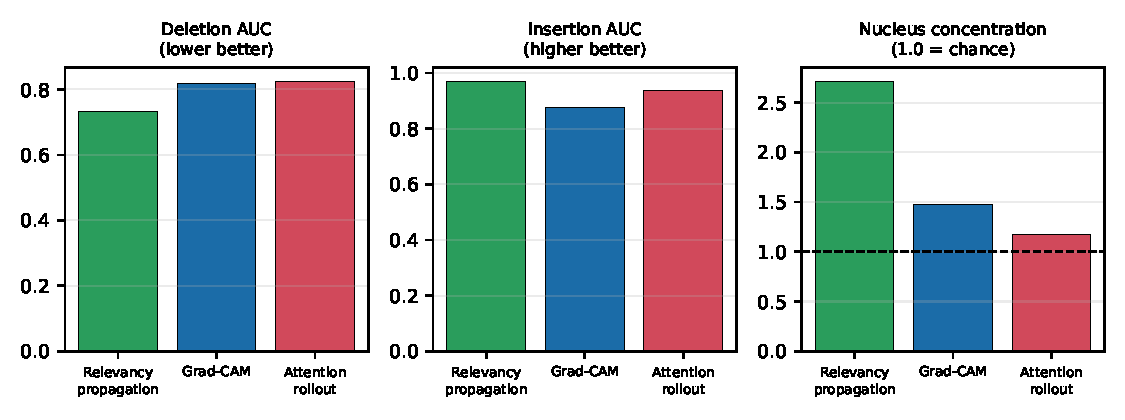
\includegraphics[width=\textwidth]{figs/p3_fig1_explainability_metrics.pdf}
\caption{Deletion AUC, insertion AUC, and nucleus concentration ratio for
the three explainability methods. Relevancy propagation wins on all
three, with the widest margin on nucleus concentration.}
\label{fig:explainability-metrics}
\end{figure}

Relevancy propagation wins every comparison, and by a wide margin on
nucleus concentration specifically (2.71$\times$ chance vs.\ attention
rollout's 1.18$\times$ -- barely above chance). We attribute this to a
mechanistic difference rather than measurement noise: attention rollout
is class-agnostic, an inherent disadvantage on an inherently
class-discriminative faithfulness test, while relevancy propagation is
both class-discriminative \emph{and} integrates the gradient-weighted
signal across all twelve transformer blocks.

\subsection{System-integration results}

Two proposed sub-claims about safe composition hold by construction given
this project's post-hoc-attachment architecture, and were verified rather
than assumed: temperature scaling changed \textbf{zero} argmax predictions
on the calibration split, and explainability computation is a read-only
analysis that cannot touch model weights. The moderate- and severe-shift
conditions below reuse the Herlev \cite{jantzen2005herlev} and Mendeley
LBC \cite{hussain2020mendeley} datasets from our companion cross-dataset
shift study.

\begin{table}[htbp]
\centering
\caption{Selective-prediction risk-coverage AUC (lower is better): confidence alone vs.\ conformal set size alone vs.\ combined.}
\label{tab:rq5}
\begin{tabular}{lrrr}
\toprule
Condition & Confidence only & Set size only & Combined \\
\midrule
In-distribution & \textbf{0.0050} & 0.0834 & 0.0173 \\
Herlev (moderate shift) & \textbf{0.1190} & 0.3281 & 0.1793 \\
Mendeley LBC (severe shift) & 0.3244 & 0.4395 & \textbf{0.2855} \\
\bottomrule
\end{tabular}
\end{table}

\begin{figure}[htbp]
\centering
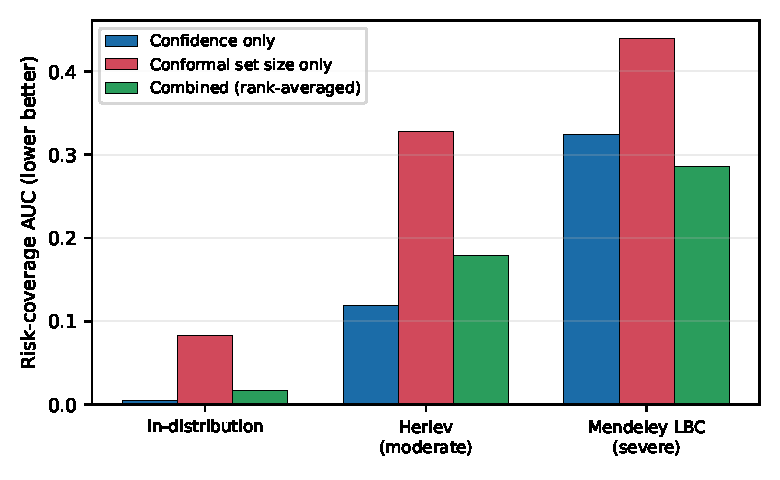
\includegraphics[width=0.85\textwidth]{figs/p3_fig3_combined_selective.pdf}
\caption{Risk-coverage AUC for confidence alone, conformal set size alone,
and the rank-averaged combination, at three conditions. Combining hurts
in-distribution and under moderate shift but helps under severe shift.}
\label{fig:combined-selective}
\end{figure}

Composition is not a uniform win. In distribution and under moderate
shift, confidence alone is already the best individual signal, and
combining it with the noisier discrete conformal-set-size signal dilutes
it. Under severe shift, however, the combined signal is the best of the
three, beating confidence alone. This mirrors the shape of our companion
uncertainty-method finding (no single choice wins everywhere), now
extended to combinations of signals.

\subsection{Resource efficiency and deployment robustness}

Across a 12-model registry, EfficientNet-Lite0 (3.38M params, 0.77G
FLOPs) has more than 4$\times$ ResNet-50's CPU latency (137.7ms vs.\
32.0ms) despite ResNet-50 having roughly 10$\times$ the FLOPs. Even
EfficientViT-M0, the overall winner on params+FLOPs+accuracy, is not the
fastest model in wall-clock CPU terms: DeiT-Tiny (15.4ms) and LeViT-128
(17.5ms) are both faster despite 10--14$\times$ more FLOPs. EfficientViT-M0,
evaluated under synthetic JPEG compression, Gaussian blur, and
brightness/contrast shift, degrades gracefully under all three, but
Gaussian blur is by far the most damaging -- costing 32.8 points of
balanced accuracy at its most severe tested level, roughly double JPEG's
worst case (15.5 points) or brightness/contrast's (18.1 points). A
synthetic OOD sanity check shows mean confidence dropping from 0.985 (real
in-distribution images) to 0.743 (OOD) -- real and meaningful, but far
above the 0.20 chance level for this 5-class task. On CPU, a bare DeiT-Tiny
forward pass has a median latency of 49.6ms; a prediction that also
returns a relevancy-propagation explanation costs 164.1ms -- about
3.3$\times$ the bare-prediction cost.

\begin{figure}[htbp]
\centering
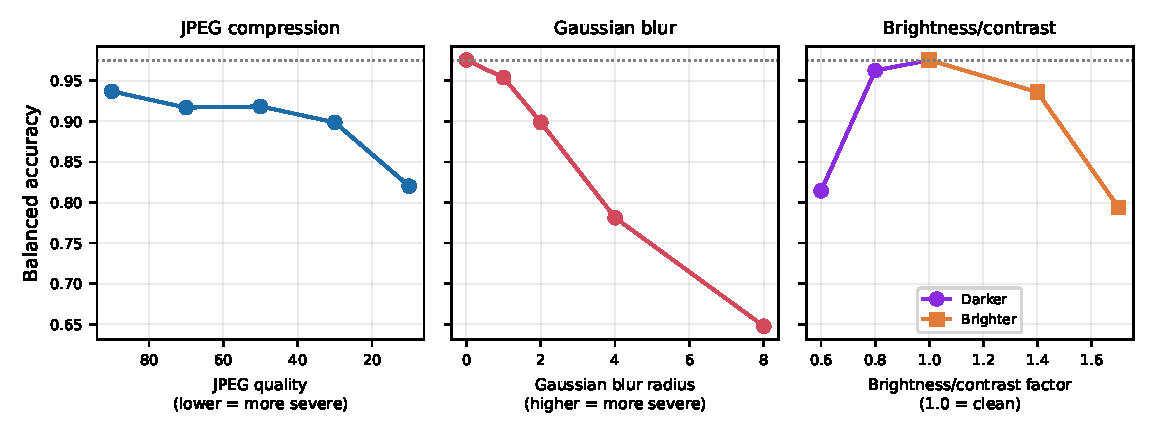
\includegraphics[width=\textwidth]{figs/p3_fig2_degradation_curves.pdf}
\caption{Balanced accuracy vs.\ corruption severity for three synthetic
degradations (EfficientViT-M0, SIPaKMeD test set). The dotted line marks
the clean baseline (0.975). Gaussian blur causes the steepest decline.}
\label{fig:degradation-curves}
\end{figure}

\section{Discussion}

Two threads run through this study. First, explainability method choice
produced the cleanest, most unambiguous result so far -- relevancy
propagation wins every metric, with no condition-dependent flip -- while
uncertainty method choice and uncertainty-signal composition both
produced conditional, no-single-winner results. This asymmetry suggests
that for this task and backbone family, picking the right explainability
method is a more reliably beneficial engineering decision than picking
(or combining) the right uncertainty-quantification method, where the
honest answer is ``it depends on the operating condition.'' Second, every
efficiency and robustness claim required direct measurement to be
trusted: FLOP count did not predict CPU latency; and OOD confidence
dropped only partially, not to the clean near-chance level a reader might
assume from an ``OOD detection'' framing.

\section{Threats to Validity}

\textbf{Internal validity.} The explainability comparison (Table~1) uses
50 test images, 10 per class, from one fixed stratified sample; a
different sample could shift the exact deletion/insertion/nucleus-
concentration numbers, though the margin by which relevancy propagation
wins on all three metrics is large enough that a resampling-driven
reversal of the ranking is unlikely. The OOD sanity check's 25-image
sample is smaller still, and its qualitative conclusion (confidence drops
but not to chance) should be treated as suggestive rather than a precise
estimate for this reason. CPU latency figures (Section~4.4) were measured
on one shared consumer laptop rather than isolated benchmark hardware; a
$\sim$30\% run-to-run swing was observed for the same model, so the exact
3.3$\times$ explanation-cost multiplier should be read as approximate, not
a precise constant.

\textbf{External validity.} All results use a single backbone (DeiT-Tiny)
chosen specifically because relevancy propagation is defined for standard
multi-head self-attention transformers and not for EfficientViT-M0's
hybrid design; whether the explainability ranking, the selective-
prediction composition result, or the degradation/OOD findings transfer
to a hybrid conv+attention backbone, or to a different medical imaging
task entirely, is untested. Single-institution data (SIPaKMeD,
$\sim$4{,}000 images) throughout.

\textbf{Construct validity.} Deletion/insertion AUC and nucleus
concentration ratio are both well-established or directly interpretable
metrics (Section~3.3), reducing the risk that the explainability ranking
is an artifact of an unusual scoring choice; using SIPaKMeD's own
expert-marked nucleus polygons as ground truth, rather than a
segmentation model's derived output, specifically avoids compounding this
paper's evaluation with a second model's own errors. No clinical or
expert-review validation of explanation localization fidelity was
performed -- agreement with a nucleus boundary is not equivalent to a
cytotechnologist judging an explanation clinically meaningful, a
distinction stated explicitly rather than implied away.

\section{Limitations}

Backbone mismatch: the explainability and system-integration results use
DeiT-Tiny, not the efficiency benchmark's overall winner, EfficientViT-M0,
since relevancy propagation is not defined for the latter; whether these
results transfer to a hybrid conv+attention backbone is untested.
Single-institution, small-scale data (SIPaKMeD, $\sim$4{,}000 images). CPU
latency measured on one shared consumer laptop, not dedicated hardware;
a $\sim$30\% run-to-run swing was observed for the same model, though
relative ordering across models was stable. OOD sanity check uses a
small, synthetic sample (25 images) rather than a natural out-of-domain
dataset. No clinical or expert-review validation of explanation
localization fidelity.

\section{Conclusion}

Three properties of one trustworthy-AI pipeline, tested side by side, do
not resolve alike. Relevancy propagation is a clearly better
explainability method than attention rollout or Grad-CAM for this
cervical cytology classifier, on both behavioral faithfulness and real
expert-annotated localization ground truth -- a clean, condition-
independent result. Composing two uncertainty signals for selective
prediction, by contrast, helps only under the specific condition where
the better individual signal was already failing -- a conditional result
that would have been reported backwards by an evaluation run under only
one shift severity. Resource-efficiency and robustness claims for
lightweight vision transformers resolve only under direct measurement,
in both directions: FLOP-efficient does not mean latency-efficient, and
``confidence drops on OOD input'' does not mean ``confidence reaches a
safe abstention level.'' No single verification strategy -- pick the best
method once, assume composition helps, trust an architectural efficiency
claim -- would have correctly characterized all three properties of this
one pipeline; each required its own test, on its own terms.

\begin{thebibliography}{99}

\bibitem{chefer2021transformer}
Chefer, H., Gur, S., Wolf, L.: Transformer interpretability beyond
attention visualization. In: CVPR (2021)

\bibitem{abnar2020quantifying}
Abnar, S., Zuidema, W.: Quantifying attention flow in transformers. In:
ACL (2020)

\bibitem{selvaraju2017gradcam}
Selvaraju, R.R., Cogswell, M., Das, A., Vedantam, R., Parikh, D., Batra,
D.: Grad-CAM: Visual explanations from deep networks via gradient-based
localization. In: ICCV (2017)

\bibitem{gal2016dropout}
Gal, Y., Ghahramani, Z.: Dropout as a Bayesian approximation:
Representing model uncertainty in deep learning. In: ICML (2016)

\bibitem{lakshminarayanan2017ensembles}
Lakshminarayanan, B., Pritzel, A., Blundell, C.: Simple and scalable
predictive uncertainty estimation using deep ensembles. In: NeurIPS (2017)

\bibitem{sensoy2018evidential}
Sensoy, M., Kaplan, L., Kandemir, M.: Evidential deep learning to
quantify classification uncertainty. In: NeurIPS (2018)

\bibitem{petsiuk2018rise}
Petsiuk, V., Das, A., Saenko, K.: RISE: Randomized input sampling for
explanation of black-box models. In: BMVC (2018)

\bibitem{guo2017calibration}
Guo, C., Pleiss, G., Sun, Y., Weinberger, K.Q.: On calibration of modern
neural networks. In: ICML (2017)

\bibitem{touvron2021deit}
Touvron, H., Cord, M., Douze, M., Massa, F., Sablayrolles, A., J\'egou,
H.: Training data-efficient image transformers \& distillation through
attention. In: ICML (2021)

\bibitem{jantzen2005herlev}
Jantzen, J., Norup, J., Dounias, G., Bjerregaard, B.: Pap-smear benchmark
data for pattern classification. In: Proceedings of Nature Inspired Smart
Information Systems (NiSIS), pp.\ 1--9 (2005)

\bibitem{hussain2020mendeley}
Hussain, E., Mahanta, L.B., Borah, H., Das, C.R.: Liquid based-cytology
Pap smear dataset for automated multi-class diagnosis of pre-cancerous
and cervical cancer lesions. Data in Brief 30, 105589 (2020)

\bibitem{mohiuddin2025}
Mohiuddin, A.B., Rahman, M.M., et al.: Accelerated and accurate cervical
cancer diagnosis using a novel stacking ensemble method with explainable
AI. In: International Conference on Quantum Photonics, Artificial
Intelligence (2025)

\bibitem{rahman2026maizeformerx}
Rahman, M.M., et al.: MaizeFormerX: a lightweight vision transformer with
cross-scale attention for explainable maize leaf disease diagnosis.
Scientific Reports (2026)

\bibitem{gony2026retinal}
Gony, M.N., Shuvra, S.M.K., Poudel, R., Dhakal, K., Rahman, M.M., et al.:
Dual-view semi-supervised retinal disease recognition via chromatic
structural decomposition and cross-view contrastive learning. In:
International Conference on Power, Electronics, Communications (2026)

\bibitem{ahmed2026postsurgical}
Ahmed, M., Ahmed, F., Mow, S.M., Taha, P.A., Barua, S., Rahman, M.M., et
al.: An explainable multimodal AI framework with reinforcement learning
for post-surgical clinical decision support. medRxiv (2026)

\end{thebibliography}
\end{document}
